% DO NOT COMPILE THIS FILE DIRECTLY!
% This is included by the other .tex files.

\begin{frame}[t,plain]
\titlepage
\end{frame}

\begin{frame}[t]{Motivating Problem I}
\begin{itemize}
\item How many sinusoids are in this data?
\item Also, what are their periods, amplitudes and phases?
\end{itemize}
\begin{center}
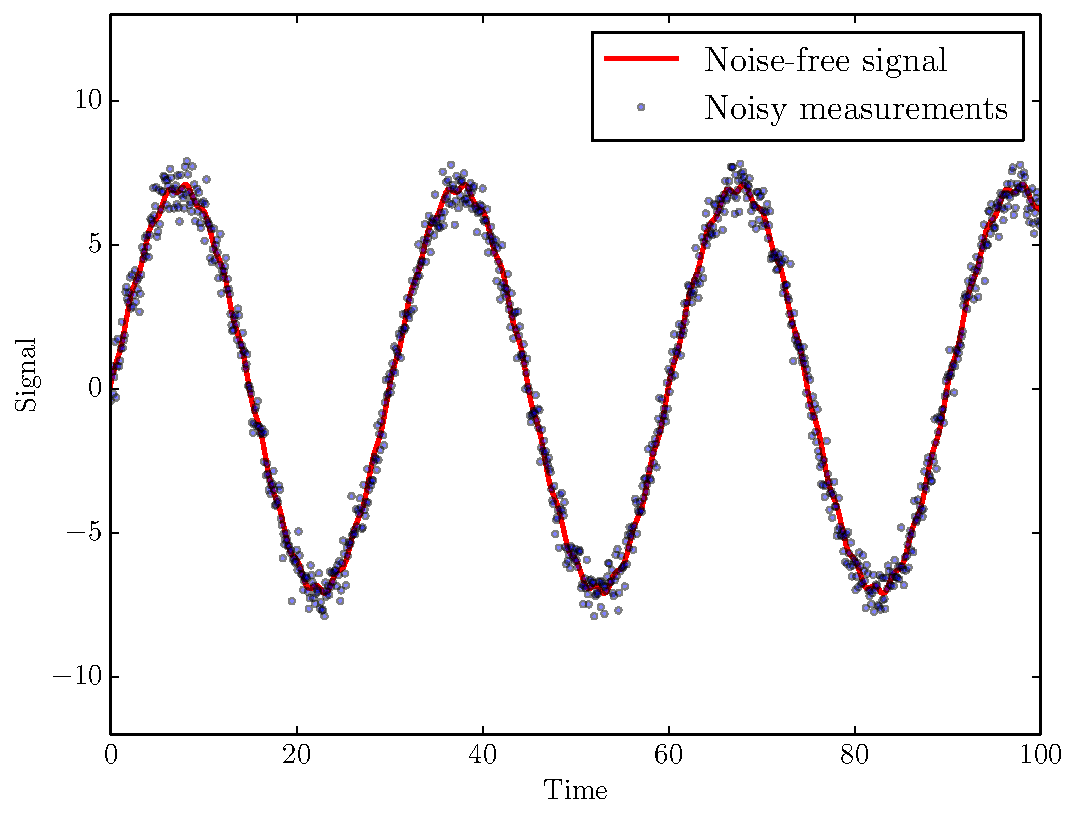
\includegraphics[scale=0.35]{sinewave_data.pdf}
\end{center}
\end{frame}

\begin{frame}[t]{Motivating Problem II}
\begin{itemize}
\item How many galaxies are in this data?
\item Also, what are their positions, sizes, orientations, etc?
\end{itemize}
\begin{center}
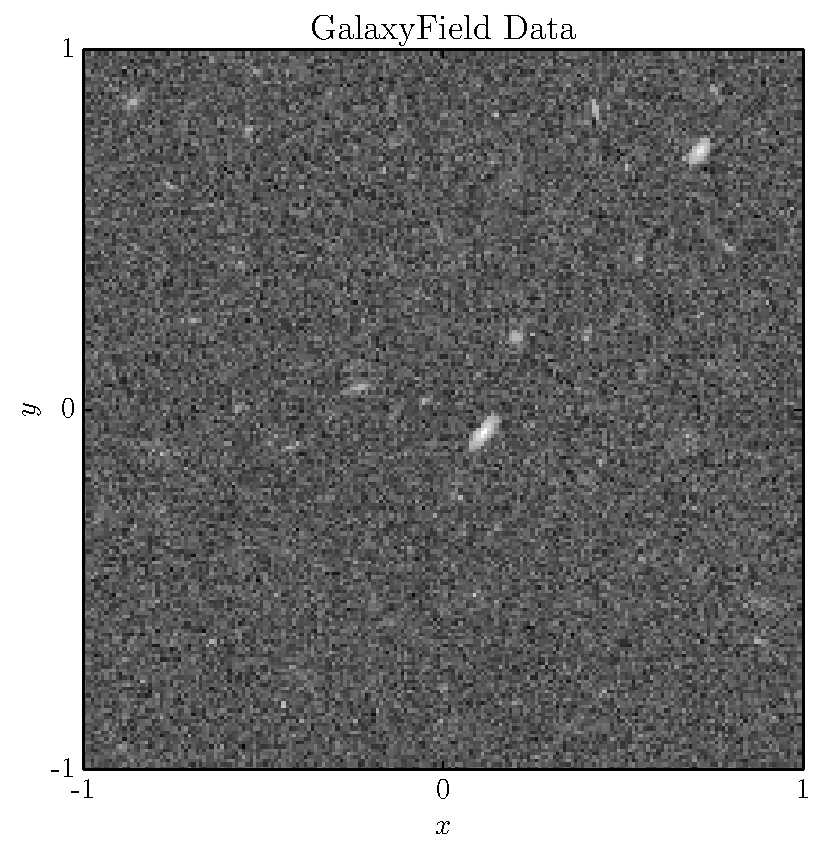
\includegraphics[scale=0.35]{../Paper/galaxyfield_data.pdf}
\end{center}
\end{frame}


\begin{frame}[t]{Similarities}
\begin{itemize}
\item Many problems (such as the previous two) have this structure:
\vspace{20pt}
  \begin{itemize}
  \setlength{\itemsep}{20pt}
  \item There are $N$ objects in a region, and we don't know the value of $N$
  \item Each object has properties $\mathbf{x}_i$
  \item We have some data $\mathcal{D}$ which we want to use to infer both $N$
        and $\{\mathbf{x}_i\}_{i=1}^N$.
  \end{itemize}
\end{itemize}
\end{frame}



\begin{frame}[t]{Bayesian Inference 101}
Bayesian Inference is a unified framework for solving inference problems.
We need the following ingredients:

\begin{itemize}
\setlength{\itemsep}{20pt}
\item A {\bf hypothesis space} describing the set of possible answers to our
question (``parameter space'' in fitting is the same concept).
\item A {\bf prior distribution} $p(\theta)$ describing how plausible
each of the possible solutions is, not taking into account the data.
\item A {\bf sampling distribution} $p(D | \theta)$ describing our knowledge
about the connection between the parameters and the data. When $D$ is known
this is a function of $\theta$ called the {\bf likelihood}.
\end{itemize}

\end{frame}


\begin{frame}[t]{Bayesian Inference 101}
The data helps us by changing our prior distribution to the {\bf posterior
distribution}, given by
\begin{eqnarray}
p(\theta | D) &=& \frac{p(\theta) p(D|\theta)}{p(D)}
\end{eqnarray}
where the denominator is the normalisation constant, usually called either
the {\bf marginal likelihood} or the {\bf evidence}.
\begin{eqnarray}
p(D) &=& \int p(\theta)p(D|\theta) \, d\theta.
\end{eqnarray}

\end{frame}

\begin{frame}[t]{Posterior Distribution vs. Maximum Likelihood}
The practical difference between these two concepts is greater in higher
dimensional problems.
\begin{center}
\includegraphics[scale=0.4]{bayes.pdf}
\end{center}
\end{frame}



\begin{frame}[t]{Computation: Markov Chain Monte Carlo}
To explore the posterior distribution, the Metropolis algorithm is a standard
technique:

\begin{itemize}
\item Start at some point $\theta$ in the hypothesis space.
\item Loop\\
$\{$
  \begin{itemize}
  \item Generate {\bf proposal} from some distribution $q(\theta' | \theta)$
  (e.g. slightly perturb the current position).
  \item With probability$^*$ $\alpha = \min\left(1, \frac{p(\theta')p(D|\theta')}{p(\theta)p(D|\theta)}\right)$, accept the proposal (i.e. replace $\theta$ with $\theta'$).
  \item Otherwise, stay in the same place.
  \end{itemize}
$\}$
\end{itemize}
\end{frame}


\begin{frame}[t]{What sampling gives us}
\begin{columns}[T]
\begin{column}{0.4\textwidth}
  \begin{itemize}
  \setlength{\itemsep}{20pt}
  \item {\bf Marginalisation} becomes trivial
  \item We can quantify all uncertainties we might be interested in
  \end{itemize}
\end{column}
\hfill
\begin{column}{0.55\textwidth}
  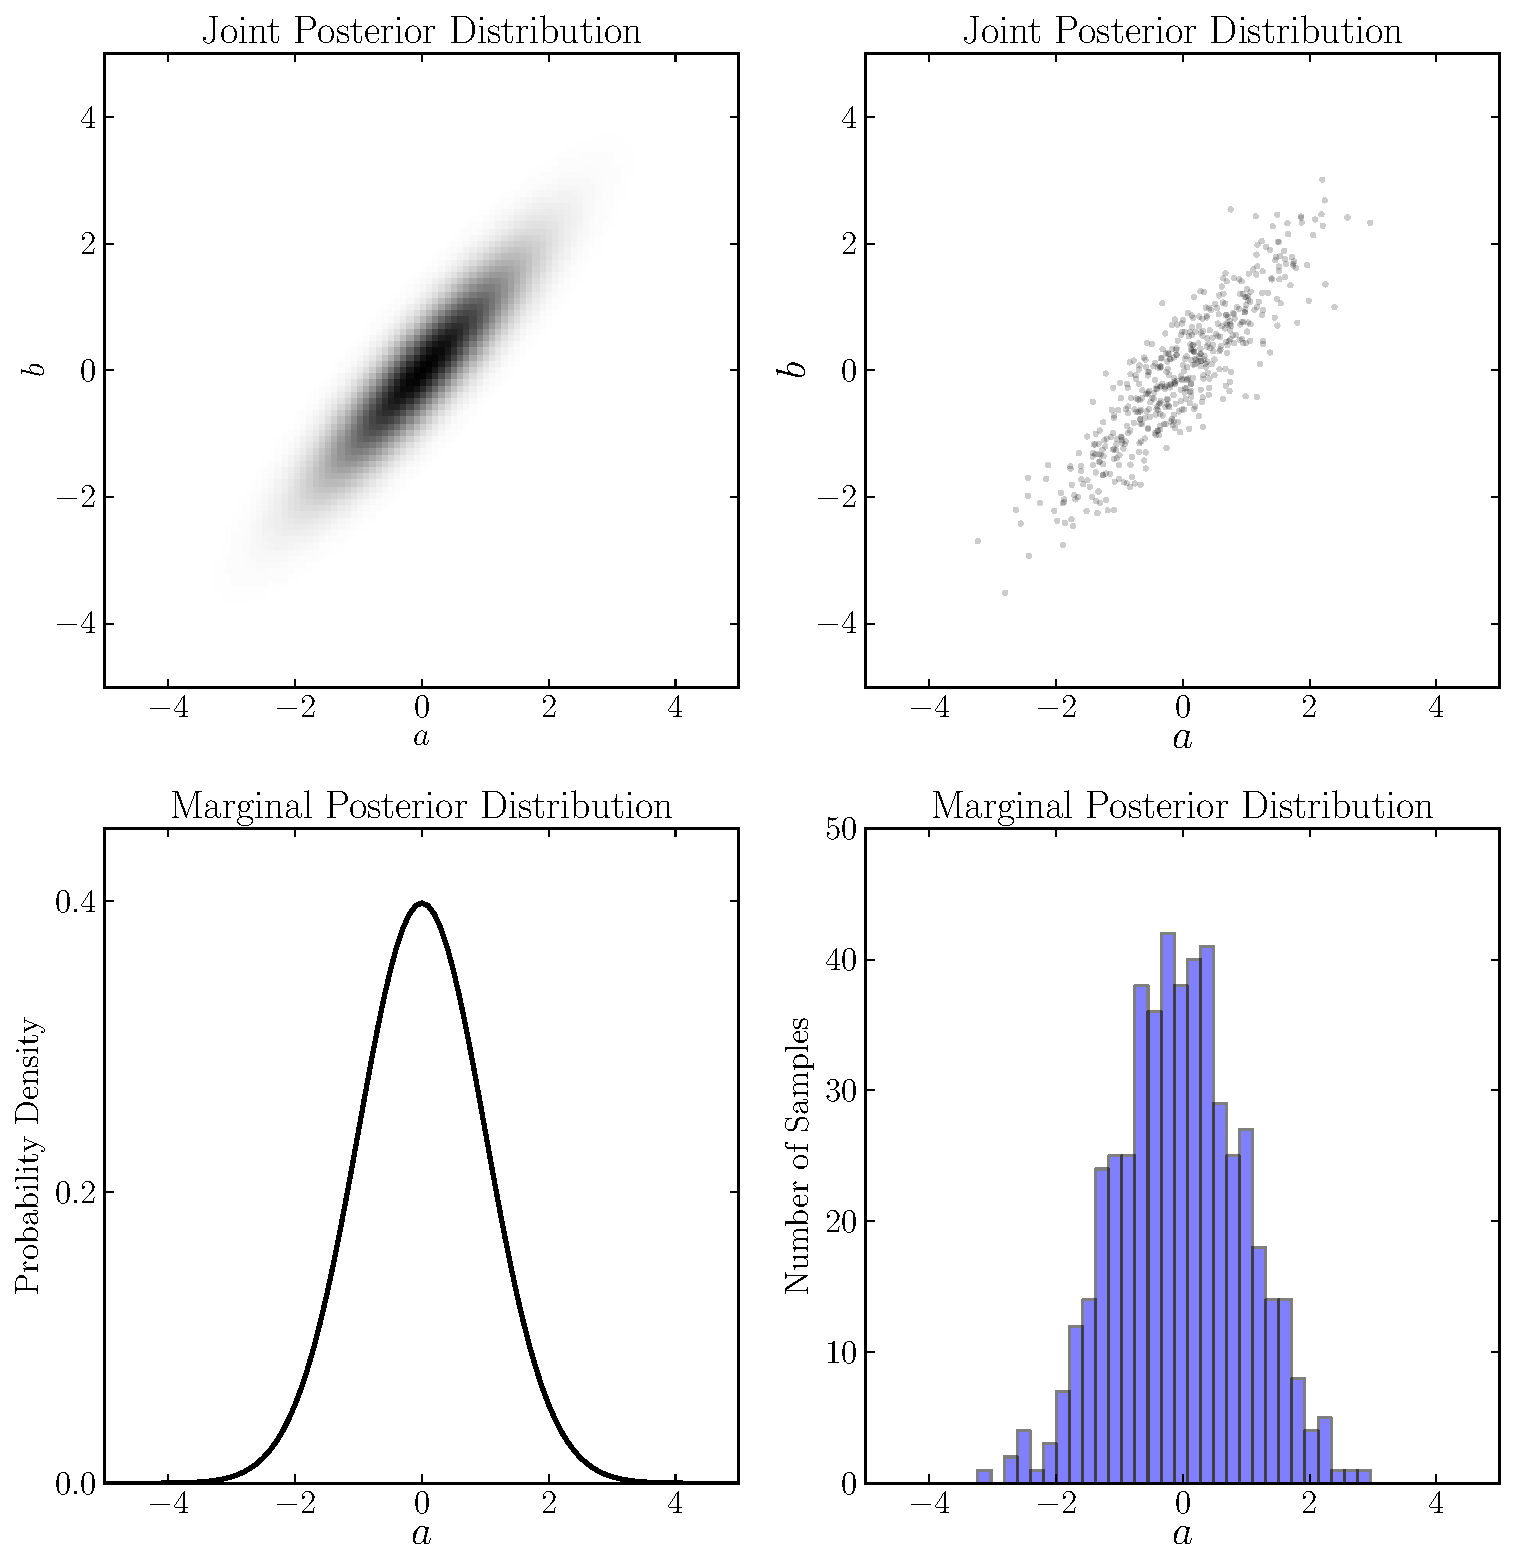
\includegraphics[scale=0.25]{marginalisation.pdf}
\end{column}

\end{columns}
\end{frame}

\begin{frame}[t]{Birth and Death}
For problems of unknown dimensionality, the hypothesis space is the union
of several fixed-dimension hypothesis spaces.


\end{frame}



